\documentclass[10pt]{article}
\usepackage[a4paper,margin=2cm]{geometry}
\usepackage[T1]{fontenc}
\usepackage{lmodern}
\usepackage{microtype}
\usepackage{amsmath,amssymb}
\usepackage{booktabs}
\usepackage{graphicx}
\usepackage{xcolor}
\usepackage{caption}
\usepackage{subcaption}
\usepackage{enumitem}
\usepackage{listings}
\usepackage{multirow}
\usepackage{siunitx}
\usepackage[hidelinks]{hyperref}
\usepackage[numbers,sort&compress]{natbib}

\captionsetup{font=small,labelfont=bf,skip=4pt}
\setlist{itemsep=1pt,topsep=2pt,parsep=0pt,leftmargin=*}
\setlength{\parskip}{2pt}
\lstset{basicstyle=\ttfamily\scriptsize,columns=fullflexible,frame=single,framerule=0.3pt,
        breaklines=true,keywordstyle=\color{blue!60!black},commentstyle=\color{gray},language=Python,
        xleftmargin=2pt,xrightmargin=2pt}
\newcommand{\obs}{\textsc{Observed.}~}
\newcommand{\interp}{\textsc{Interpretation.}~}
\newcommand{\spec}{\textsc{Speculation.}~}
\newcommand{\up}[1]{\textcolor{green!45!black}{#1}}
\newcommand{\dn}[1]{\textcolor{red!70!black}{#1}}

\title{\vspace{-1.2cm}Masking Geometry and Noise Robustness in a Tiny I-JEPA on CIFAR-10:\\
a Controlled Study\vspace{-0.2cm}}
\author{Mohammad Al Fahim \\ \small HackerRank Deep Learning Research Engineer assignment}
\date{\small November 2026}

\begin{document}
\maketitle
\vspace{-0.6cm}

\begin{abstract}
\noindent
We reproduce the Tiny I-JEPA of \texttt{keon/jepa}~\cite{keon2023jepa} on fixed CIFAR-10 splits and evaluate its frozen
context encoder with a linear probe under occlusion and Gaussian noise. The baseline does not collapse and its clean accuracy
keeps rising with training (35.2\% at the required 500 steps, $48.9{\pm}0.4$\% at 15k steps over 5 seeds), but its accuracy at
noise $\sigma{=}0.15$ \emph{falls} after $\sim$2k steps, to $22.2{\pm}1.0$\%, below a frozen random encoder ($26.6{\pm}1.3$\%).
The latent loss is minimal at step 700, when the features are still at random-encoder level, and its first drop is learnt
from target positions alone: lower loss does not mean better features (H2 supported). For the research change we test masking
geometry (H1) with six samplers, five of them with fixed token counts. One large contiguous target block is the
most noise-robust geometry: $27.5{\pm}2.3$\% at $\sigma{=}0.15$ against $22.2{\pm}1.0$\% for the baseline (5 seeds each),
keeping 55\% instead of 45\% of its clean accuracy, with +2.3/+2.8 points at 25\%/40\% occlusion. Its ablation with the
same token counts but many small scattered target blocks is the least robust (17.0\%, 34\% of clean). With one large hole
most targets are far from the visible context and must be inferred from image-level content; with small blocks every target
has context one patch away, and the model solves the task from local detail and target positions: the scattered encoder
halves the image-specific feature variance, and its held-out loss depends much less on the image's own context and is much
closer to a position-only prediction. No geometry, however, lifts noise accuracy clearly above a frozen random encoder. A probe trained on a mix of clean and noisy images recovers 39.6\% at $\sigma{=}0.15$ from the \emph{same} frozen
baseline encoder without losing clean accuracy (48.8\%): the class information survives and only moves in feature space. Adding noise to the context-encoder input
during pretraining (targets stay clean) gives 41.9\% with the standard clean probe at a 1.4-point clean cost. The best
supported answer to the final question: the bottleneck is not collapse or context size; mask geometry decides how much the
encoder relies on local detail and positions, and hence how fragile it is to noise, but the main limit is the absence of any
invariance pressure in the objective, which a clean-only probe protocol exposes.
\end{abstract}

%=====================================================================================================
\section{Architecture and code-level explanation (A1)}
\label{sec:arch}
All line numbers refer to \texttt{ijepa.py} at commit \texttt{d55bab7b}; the full write-up is in
\texttt{docs/A1\_code\_explanation.md}.

\textbf{Patch tokens and the encoder.} The encoder follows the ViT architecture with hidden dimension 128, depth 6 and 4 heads. 
\texttt{patch\_proj} is a $4{\times}4$/stride-4 convolution, so a $32{\times}32$
image becomes $8{\times}8$ grid: 64 tokens of dimension 128 (row-major; token $p$ is patch $(\lfloor p/8\rfloor, p \bmod 8)$). A fixed 2-D
sin--cos table is added and used for position embedding (L59, L67). Given indices \texttt{idx} (L66--69), the encoder \emph{gathers} only those tokens
before the 6 pre-LN transformer blocks, so masked patches are physically absent (no mask token, no attention to them).
Because kernel = stride, gathering after the convolution cannot leak target pixels. Evaluation calls the
encoder with \texttt{idx=None} and mean-pools the 64 output features (no CLS token).

\textbf{\texttt{sample\_ijepa\_masks()} (L91--117).} Per \emph{batch} uses one target shape (scale $U(0.15,0.20)$, aspect
$U(0.75,1.5)$, i.e.\ $3{\times}3$, $3{\times}4$, $4{\times}3$ or rarely $4{\times}4$ patches) and one square context shape
(scale $U(0.85,1)$, $7{\times}7$ or $8{\times}8$) are drawn. Per \emph{image}, 4 target blocks are placed uniformly (they may
overlap; their union is $\approx$32 patches), then the context block is placed and every target patch is removed from it
% (retry $\le$10 times for $\ge$4 patches; a fallback to \texttt{[0]} could leak a target patch on tiny grids, so we wrap the sampler in a leak check). 
Finally every context patch is randomly subsampled to the \emph{batch minimum} length, so the context
length depends on the batch size ($\approx$29 tokens at $B{=}1$, 20 at $B{=}64$, 19 at $B{=}256$) and varies between steps
(4--31 at $B{=}64$). The predictor must produce $4{\times}\approx 11{=}45$ target tokens from $\approx$20 visible context features.

\textbf{Predictor and latent targets.} The predictor follows a narrower version of the encoder architecture with hidden dimension 64, depth 4 and 4 heads. 
The predictor (L74--88) projects context features $128{\to}64$, adds their positions,
appends one shared learnable mask token plus position for each target patch, runs 4 blocks, and maps the target slots back
to 128-d. It is called once per target block. Its target is $\mathrm{LN}(f_{\bar\theta}(x))$ at the target positions from
the EMA encoder applied to the \emph{full} image (masking the encoder \emph{output}, as in~\cite[Tab.~11]{assran2023ijepa}).
Predicting features instead of pixels lets the model discard unnecessary pixel detail; the paper reports 66.9\% vs
40.7\% (1\% ImageNet) for feature vs pixel targets~\cite[Tab.~7]{assran2023ijepa}.

\textbf{EMA and stop-gradient (L37--40, L127--153).} The target encoder is a frozen deep copy (\texttt{requires\_grad=False},
forward under \texttt{no\_grad}, not in the optimizer) updated only by $\bar\theta\leftarrow m\bar\theta+(1-m)\theta$ after each
optimizer step, $m$: $0.996\to1$. With this schedule the target still carries weight $\prod_s m_s\approx e^{-1}\approx 0.37$
on its random initialisation after 500 steps (0.13 after 1k, $\approx$0 after 5k). Nothing in the loss prevents feature collapse and the
asymmetry (predictor + stop-gradient + EMA) is the only protection
% , and LN on the targets does not remove a shared constant.

\textbf{Low loss vs collapse vs poor accuracy.} These are different measurements. The loss is relative to a moving target and
can be small because the target is \emph{easy} (near-random, low-rank or position-dominated). Collapse means features stop
varying across images (complete) or vary in few directions (dimensional), so we measure per-feature std, effective
rank~\cite{roy2007effrank}, top-1 singular-value share and mean pairwise cosine. Poor accuracy means that the feature reprsentations are not
linearly class-separable. To expose a \emph{positional shortcut} we report two content-ablated held-out losses: context taken
from \emph{another} image, and a content-free predictor that outputs the per-position mean (loss evaluates the target position features and is calculated against the per-position mean target features and the target features. So if the loss value is low: per-position target features are the position biased features, and if the loss is high, then target features highly depend on the image features).
If the heldout-latent loss on validation set is close to the content-free heldout loss, then the predictor returns features highly biased on the target positions.

\textbf{What we modify and what must stay invariant.} We replaced \texttt{train()} by a step-limited loop and changed only
the mask sampler (Part B) and, in Sec.~\ref{sec:noise}, the context-encoder input. Invariants (all tested,
App.~\ref{app:tests}): valid, disjoint context/target indices; rectangular batches; context encoder sees only visible tokens;
target under \texttt{no\_grad}, absent from the optimizer and changed only by EMA (applied after \texttt{opt.step()});
identical loss (tested equal to the upstream inline code); frozen encoder during probing; identical splits and corruption
tensors (hash-checked) for every model.

%=====================================================================================================
\section{Pipeline and evaluation protocol (A2)}
\label{sec:pipeline}
\textbf{Data.} From the official CIFAR-10~\cite{krizhevsky2009cifar} training split we draw, with seed 0, disjoint
class-stratified subsets: 10{,}000 unlabelled pretraining, 2{,}000 probe-training and 1{,}000 validation images; 2{,}000
test images come from the official test split (seed 1). Indices are stored in \texttt{results/splits.json}
(fingerprint \texttt{f8c34b6bbf7f644f}, checked by every notebook).

\textbf{Stress tests.} Applied once, in $[0,1]$ pixel space before normalisation, to the same 2{,}000 test images.
Occlusion: one square of side 10/16/20 px (9.8/25.0/39.1\% of the area) at a uniform random position, filled with the
CIFAR-10 channel mean (0 after normalisation); seeds 1000--1002. Gaussian noise: $x+\mathcal N(0,\sigma^2)$, $\sigma\in\{0.05,0.15\}$,
clipped to $[0,1]$; seeds 1010--1011. Tensor hashes are identical across all runs, so comparisons are paired.

\textbf{Training.} Unmodified upstream model, loss, optimiser (AdamW, lr $3{\times}10^{-4}$, wd 0.05 on 2-D weights, 5\%
warm-up + cosine decay scheduler), EMA schedule and augmentation (RandomResizedCrop 0.3--1), batch 64, FP32, 1{,}412{,}864 trainable
parameters. \textbf{Budgets (disclosed):} 500 steps (assignment), 5{,}000 steps (3 seeds, Part~A) and 15{,}000 steps for
every Part B/C comparison (96 epochs; $\approx$15--25 mins on one L40S, peak memory 0.26--0.33 GB). We select the final step checkpoint from all trainings for downstream evaluations.

\textbf{Probe.} We use the Frozen \emph{context} encoder, all 64 patch features, mean pooling, features standardised with probe-train
statistics, \texttt{Linear(128,10)}, AdamW, batch 256, 100 epochs; $(\mathrm{lr},\mathrm{wd})\in\{10^{-3},3{\cdot}10^{-3},10^{-2}\}\times\{0,10^{-4},10^{-2}\}$
selected on \emph{validation}; the test set is never used for selection. The probe is trained on clean images only and
applied unchanged to every test condition. Every result also reports the frozen random-initialisation encoder of the same
run as control. Curves during training use a single fixed probe setting (lr $3{\cdot}10^{-3}$, wd $10^{-4}$).

\textbf{Diagnostics.} Held-out latent loss on 1{,}000 validation images with fixed masks (seed 12345), plus the two
content-ablated variants of Sec.~\ref{sec:arch}; collapse statistics on clean test features (probe with frozen encoder trained on clean test features and evaluated for robustness during training); an \emph{oracle} probe (refit on
corrupted probe-train images for diagnosis of the failure mode only) that measures how much class information remains linearly decodable.

\textbf{Tests and engineering.} 49 pytest tests (App.~\ref{app:tests}) plus in-notebook assertions for every new sampler.
The Colab notebook \texttt{notebooks/experiment.ipynb} runs top to bottom in a fresh runtime (setup, CPU smoke test with one
batch forward/backward and one optimiser step, tests, splits, baseline/proposed/ablation, probe evaluation, robustness plots).
The experiments were developed in notebooks; all numbers below were produced by one script that executes those notebooks'
own cells headless, which reproduced every notebook result we had recorded within 0.1 points (L40S vs RTX 2080 Ti numerics).

%=====================================================================================================
\section{Baseline (A3)}
\label{sec:baseline}
\begin{table}[t]\centering\small\setlength{\tabcolsep}{3.5pt}
\caption{Baseline: frozen context encoder, clean-trained linear probe, test accuracy (\%, mean $\pm$ std over $n$ pretraining seeds). Held-out latent loss on fixed validation images and masks; feature std = mean per-feature std of pooled features; rank = effective rank (/128).}
\label{tab:baseline}
\begin{tabular}{lcccccccccc}\toprule
Encoder & $n$ & Clean & Occ 10\% & Occ 25\% & Occ 40\% & Noise .05 & Noise .15 & Loss & Feat.\ std & Rank \\\midrule
I-JEPA, 500 steps & 3 & 35.2{\scriptsize$\pm$0.5} & 33.6{\scriptsize$\pm$0.4} & 29.6{\scriptsize$\pm$1.3} & 23.5{\scriptsize$\pm$0.1} & 35.0{\scriptsize$\pm$0.7} & 31.3{\scriptsize$\pm$1.4} & 0.078 & 0.495 & 22.4 \\
I-JEPA, 5k steps & 3 & 42.9{\scriptsize$\pm$1.4} & 40.5{\scriptsize$\pm$1.4} & 32.3{\scriptsize$\pm$1.1} & 24.3{\scriptsize$\pm$1.1} & 41.6{\scriptsize$\pm$1.3} & 32.3{\scriptsize$\pm$0.5} & 0.113 & 0.549 & 51.9 \\
I-JEPA, 15k steps & 5 & 48.9{\scriptsize$\pm$0.4} & 46.1{\scriptsize$\pm$0.5} & 37.3{\scriptsize$\pm$0.8} & 28.9{\scriptsize$\pm$0.4} & 45.8{\scriptsize$\pm$0.4} & 22.2{\scriptsize$\pm$1.0} & 0.150 & 0.618 & 62.9 \\
\quad its random init & 5 & 35.1{\scriptsize$\pm$0.3} & 34.1{\scriptsize$\pm$0.9} & 29.6{\scriptsize$\pm$0.6} & 23.9{\scriptsize$\pm$0.7} & 34.2{\scriptsize$\pm$0.8} & 26.6{\scriptsize$\pm$1.3} & 0.533 & 0.380 & 23.8 \\
\midrule
\textit{Supervised ref., 5k} & 3 & 59.6{\scriptsize$\pm$0.3} & 55.0{\scriptsize$\pm$1.2} & 45.3{\scriptsize$\pm$0.7} & 35.4{\scriptsize$\pm$1.0} & 58.2{\scriptsize$\pm$0.6} & 44.6{\scriptsize$\pm$0.2} & -- & 0.824 & 64.9 \\
\bottomrule\end{tabular}\end{table}


\begin{figure}[t]
\centering
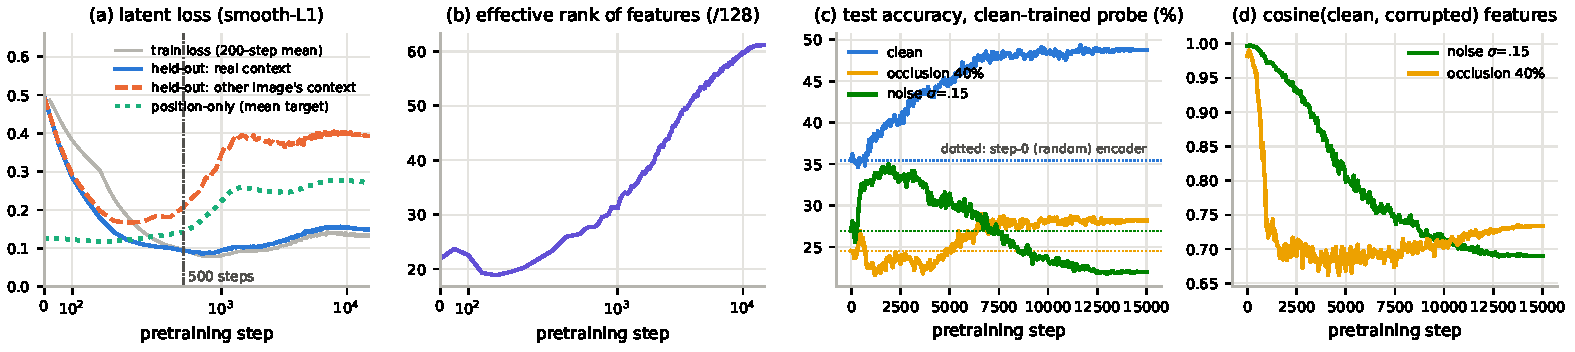
\includegraphics[width=\linewidth]{figures/fig_baseline.pdf}
\caption{Baseline dynamics (15k steps, seed 0). (a) Training loss and held-out latent loss with the real context, with
another image's context, and for a content-free predictor that outputs the per-position mean target. (b) Effective rank of
pooled features. (c) Test accuracy with a fixed clean-trained probe; dotted: the step-0 (random) encoder. (d) Cosine between
clean and corrupted features of the same image.}
\label{fig:baseline}
\end{figure}

\obs (Tab.~\ref{tab:baseline}, Fig.~\ref{fig:baseline}.) At the assignment budget of 500 steps the pretrained encoder is
indistinguishable from the frozen random encoder on clean data (35.2 vs 35.1) and on every occlusion level; only
$\sigma{=}0.15$ noise is higher (31.3 vs 26.6). Longer training is required for useful features: 42.9\% at 5k and 48.8\% at
15k steps clean (5 seeds, $\pm$0.4), always far above the random encoder (35.1\%). The supervised reference (same ViT and data,
labels used; diagnostic only) reaches 59.6\% at 5k. Noise $\sigma{=}0.15$ is the exception: 31.3\% at 500 steps, 32.3\% at 5k,
but $22.2{\pm}1.0$\% at 15k, below the random encoder's $26.6{\pm}1.3$\% (Sec.~\ref{sec:failure}).

%=====================================================================================================
\section{Hypotheses (A4)}
\label{sec:hyp}
\textbf{H1 -- masking geometry.} With per-image context and target token counts held equal to the baseline (20 visible,
32 target patches), replacing the 4 small target blocks by 1--2 large contiguous blocks raises clean-probe accuracy at
25\% and 40\% occlusion by more than the seed standard deviation without lowering clean accuracy by more than 1.4 points.
This can be falsified if the gain is within seed noise, or if the scattered-block control with the same counts gets the same
gain (then counts, not geometry, are responsible).

\textbf{H2 -- loss vs representation quality.} 
Lower latent predictions loss does not imply that the feautre representations are class-discriminative. 
This can be falsified if we observe the opposite.
% Held-out latent loss does not rank representations by probe accuracy, while
% the effective rank of the features does. \emph{Falsified} if lower held-out loss goes with higher accuracy across
% checkpoints and across variants.

%=====================================================================================================
\section{Failure-mode diagnosis}
\label{sec:failure}
\subsection{Main failure: noise robustness degrades as the representation improves}
\obs Accuracy at $\sigma{=}0.15$ rises to 35.0\% at step 1{,}900 and then falls monotonically to 22.0\% at 15k (seed 0,
fixed probe), while clean accuracy keeps rising (Fig.~\ref{fig:baseline}c). Over 5 seeds the final value is $22.2{\pm}1.0$\%,
below the random encoder ($26.6{\pm}1.3$\%). 
% Over steps $\ge$500 the Spearman
% correlation between effective rank and $\sigma{=}0.15$ accuracy is $\rho={-}0.98$ (with clean validation accuracy
% $\rho={+}0.92$). 
The cosine between clean and noisy features of the same image drops from 0.997 to 0.69
(Fig.~\ref{fig:baseline}d). The failure is not specific to our seed or masks: every one of the 6 pretrained variants in
Tab.~\ref{tab:h1} ends between 17.0\% and 31.2\% at $\sigma{=}0.15$.

\obs \emph{The information is still there} (Tab.~\ref{tab:noise}). We retrain only the linear probe, on the \emph{same
frozen} baseline encoder, with a \emph{mixed} probe-train set: in every one of the 100 probe epochs each of the 2k probe-train
images is used clean or, with probability $\tfrac12$, as a noisy copy with a fresh $\sigma{=}0.15$ draw (mask and noise
seeds disjoint from the test-noise seed). Standardisation statistics come from the clean and all noisy probe-train features,
and $(\mathrm{lr},\mathrm{wd})$ is selected on the mean of clean and noisy ($\sigma{=}0.15$) validation accuracy. This probe
gives \textbf{39.6\%} at $\sigma{=}0.15$ (+17.6 points) with unchanged clean accuracy (48.8\%), far above the same procedure
on the random encoder (31.3\%).

\interp The pretrained features of a noisy image are informative but lie in a different region of feature space than
the clean features the probe was fit on. 
% As training proceeds the encoder spends its growing rank on fine, local
% structure, which is exactly what i.i.d.\ pixel noise perturbs. 
As training proceeds, the encoder slowly starts learning the context patch features to predict the target features and 
its sensitivity to noise increases. Since we are only masking the target blocks on the input image for the context encoder,
its robustness to occlusion increases but the context feature representations are still sensitive to high noise. 
Using a larger encoder (increasing the number of transformer blocks, heads, and the hidden dimension) might help with this,
because it allows the encoder to learn more semantic features, making it more robust to high noise. 
We are also not augmenting the input images in I-JEPA (since I-JEPA proposes an augmentation-free self-supervsied pretraining method,
thereby removing the need to hand-craft augmentations with respect to the downstream task). Due to this, there is no direct supervision
for the encoder to be invariant to noise. In our pipeline the only
augmentation is RandomResizedCrop, which is no defence against pixel noise. For diagnosis, we trained the probe using the frozen baseline
context encoder with noise augmentation and observe that its robustness to noise ($\sigma{=}0.15$) increases. This means that 
noisy feature representations from the encoder are still class-discriminative and seperable, but are very sensitive to high noise when 
comparing the results against the clean-trained probe.

% This is consistent with what the paper reports about
% I-JEPA: it is trained \emph{without} hand-crafted view augmentations~\cite[Sec.~1]{assran2023ijepa}, so nothing in the
% objective asks for invariance to any perturbation, and its representations keep much of the local structure of the
% input~\cite[App.~E.1, Tab.~4]{assran2023ijepa} (it beats view-invariant methods on counting and depth). 

\subsection{Loss does not track representation quality (H2)}
\label{sec:h2}
\obs (Fig.~\ref{fig:baseline}a.) \emph{Steps 0--200:} the held-out loss falls from 0.495 to 0.179, but the loss with
another image's context falls identically (0.494 $\to$ 0.198), and the content-free per-position mean target scores
\emph{lower} than both until step $\approx$250 (0.12). \emph{Steps 250--700:} the real-context loss separates from the
other-image loss and reaches its minimum, 0.086, at step 700, while validation accuracy (37.9\%) and effective rank (28) are
still at random-encoder level. \emph{Steps $>$700:} the content-free loss rises from 0.12 to 0.27, the held-out loss rises
% to 0.149, and accuracy climbs to 51.0\% (val). 
% Over steps $\ge$500, Spearman $\rho(\text{held-out loss},\text{val acc})={+}0.65$:
% higher loss goes with \emph{better} features. 
Across the variants of Tab.~\ref{tab:h1} the loss does not rank them
either (e.g.\ scattered has the lowest loss, 0.113, but the worst noise accuracy, 17.0\% at $\sigma{=}0.15$).

\interp Early on, the EMA target encoder is still mostly its random initialisation, and a random ViT with additive sin--cos
positions produces features dominated by \emph{position}: a predictor that knows only the target position already matches
them, so the first drop of the loss is learnt from positional embeddings alone, without looking at the image. By step 500
the predictor uses some image content (real-context loss 0.078--0.094 vs 0.21 with another image's context), but the
image-dependent part of the target is small and low-rank, so it is easy to regress and carries little class information.
As the EMA target moves away from its initialisation, its features become image-specific (the content-free loss rises), the
prediction task becomes harder (loss rises) and the context encoder has to infer the target from the content of the visible
patches, which is when semantic, class-relevant features emerge. Representation quality is therefore read from the probe,
the robustness curves and the collapse diagnostics (rank 22$\to$61, top-1 singular-value share 0.73$\to$0.12, pairwise cosine
0.84$\to$0.29: no collapse), not plainly from the loss. The training latent predictor loss curve can show signs of feature 
collapse if the loss does not increase after its first dip. \textbf{H2 is supported.} Losses of different variants are not comparable
anyway, because each has its own evolving target encoder.

% \subsection{Severe occlusion: mostly missing evidence}
% \obs At 15k steps the clean-trained probe keeps 58\% of clean accuracy at 40\% occlusion (28.2/48.8); an oracle probe refit
% on occluded probe images reaches 38.4\%. At 5k steps the supervised reference loses the same fraction as I-JEPA
% (retention 0.59 vs 0.57). \interp A $20{\times}20$ px square often removes the class evidence itself (a failure no
% representation can fully avoid); the remaining gap is a probe/feature shift like the noise failure, smaller in size.

%=====================================================================================================
\section{Research change: masking geometry (Part B)}
\label{sec:partb}
\textbf{Change.} We added a sampler interface (\texttt{cfg["mask\_strategy"]}) and a \emph{fixed-count} rule (declared context and
target sizes with random selection, as in fixed-size multi-block collators): per image, positions are redrawn until the context block minus all
target blocks offers $\ge$\texttt{ctx\_size}=20 patches and the target blocks $\ge$\texttt{tgt\_size}=32 patches; then exactly
20 and 32 indices are drawn uniformly. This removes the batch-minimum trimming, so every candidate below sees the
\emph{same} token counts at every step and batch size (the baseline's 45 target tokens contain $\approx$32 distinct patches;
20+45 distinct patches do not fit on 64). As in upstream I-JEPA, each target block is predicted as its own set and the
losses are averaged
% : with $n$ blocks, $32/n$ tokens are drawn from each block (4$\times$8, 2$\times$16, or one set of 32 for
% \texttt{1\_large}), so a patch covered by two overlapping blocks can be a target twice; \texttt{scattered} predicts each of its
% 6--16 small blocks whole (32--36 tokens). 
Core code is in
App.~\ref{app:diff}; masks are illustrated in Fig.~\ref{fig:masks}. Parameters are unchanged by every sampler; runtime and
memory grow only with the number of target sets (Sec.~\ref{sec:partc}).

\textbf{Block shapes (all strategies).} 
% As upstream, a scale $s$ and an aspect ratio $r$ become a block of $h{\times}w$
% patches with $h=\mathrm{round}\sqrt{64\,s\,r}$, $w=\mathrm{round}\sqrt{64\,s/r}$ (\texttt{\_bsize}, clipped to 1--8).
One target-block shape and one context-block shape are drawn per \emph{batch}; block positions are drawn per \emph{image},
uniformly over the grid. The context block is always square ($r{=}1$, $s\sim U(0.85,1)$): $8{\times}8$ in 81\% and
$7{\times}7$ in 19\% of batches, and the visible context is the context block minus every target patch. Target blocks use
$r\sim U(0.75,1.5)$ and a strategy-specific scale (Tab.~\ref{tab:masks}). Under the fixed-count rule a target shape with
$n\,h\,w<32$ is redrawn at once, and if one image finds no valid position within 200 draws, the batch's shapes are redrawn
(0.09 times per batch for \texttt{1\_large}, 0.14 for \texttt{2\_large\_nonoverlap}, 0 otherwise).

\begin{table}[t]\centering\small\setlength{\tabcolsep}{3pt}
\caption{Masking strategies. Target-block scale $s$ (aspect $r\sim U(0.75,1.5)$ for all; context block: square, $s\sim
U(0.85,1)$, $8{\times}8$ or $7{\times}7$), the resulting target shapes $h{\times}w$ with their share of batches (measured over
400 batches of 64), the placement rule, the context rule and the target sets (one loss term each).}
\label{tab:masks}
\resizebox{\linewidth}{!}{\begin{tabular}{llllll}\toprule
Strategy & Blocks, scale $s$ & Target shapes (\% of batches) & Placement & Context tokens & Target sets \\\midrule
Baseline (upstream) & 4, $U(0.15,0.20)$ & $4{\times}3$ 54, $3{\times}3$ 27, $3{\times}4$ 19, $4{\times}4$ 1 & may overlap & batch minimum, 4--31 & 4 whole blocks (9--16) \\
\texttt{1\_large} & 1, $U(0.52,0.62)$ & $7{\times}5$ 42, $6{\times}6$ 33, $7{\times}6$ 9, $6{\times}7$ 7, $5{\times}7$ 7, $8{\times}5$ 3 & -- & exactly 20 & 1 set of 32 from the block \\
\texttt{scattered} & until $\ge$32 patches, $U(0.04,0.07)$ & $2{\times}2$ 88, $2{\times}1$ 11, $1{\times}2$ 1, $3{\times}2$ 1 & disjoint & exactly 20 & every block whole: 8$\times$4, 16$\times$2, 6$\times$6 \\
\texttt{2\_large\_overlap} & 2, $U(0.30,0.40)$ & $5{\times}4$ 31, $5{\times}5$ 28, $6{\times}4$ 20, $4{\times}5$ 15, other 6 & may overlap & exactly 20 & 2 sets of 16, one per block \\
\texttt{2\_large\_nonoverlap} & 2, $U(0.25,0.32)$ & $5{\times}4$ 46, $4{\times}4$ 35, $4{\times}5$ 19 & disjoint & exactly 20 & 2 sets of 16, one per block \\
overlap cap $<$25\% & 4, $U(0.15,0.20)$ & $4{\times}3$ 50, $3{\times}3$ 27, $3{\times}4$ 23, $4{\times}4$ 1 & $|A\cap B|/|A|<0.25$ & batch minimum $\le$20, 12--20 & 4 sets of 8, one per block \\
\bottomrule\end{tabular}}
\end{table}

\textbf{Baseline (upstream).} Per image, 4 blocks of the batch's shape (9--16 patches) are placed independently and may overlap
(union $\approx$32 patches); the context block is placed and the target patches are removed from it.
% (its position is redrawn up to 10 times until $\ge$4 patches remain). 
All context lists are then randomly subsampled to the batch minimum
(mean 20.3, range 4--31 at $B{=}64$), and every block is a target set with all its patches.
% (36, 48 or 64 target tokens).

\textbf{Proposed: \texttt{1\_large}.} One block of 35--42 patches ($s\sim U(0.52,0.62)$; the 30-patch shapes $6{\times}5$ and
$5{\times}6$ are rejected because they cannot supply 32 targets), so more than half of the image is hidden as one
contiguous region. Positions are redrawn until the context block minus the block keeps $\ge$20 patches; then exactly 20
context and 32 target patches (of the 35--42) are drawn uniformly, and the 32 are one target set. With one large hole most
target patches are several patches away from any visible patch, so they can only be predicted from image-level content.

\textbf{Ablation: \texttt{scattered}.} Per batch one \emph{small} shape is drawn ($s\sim U(0.04,0.07)$): $2{\times}2$ in 88\%
of batches, $2{\times}1$ or $1{\times}2$ in 12\%, rarely $3{\times}2$. The \emph{number} of blocks is not set; it follows from the
target budget. Per image, blocks of that shape are added one at a time, each at a uniform position among those that share no
patch with the earlier blocks, until their union covers $\ge$\texttt{tgt\_size}=32 patches. Because the blocks are disjoint
and of equal size $a=h\,w$, this takes exactly $\lceil 32/a\rceil$ blocks: 8 blocks of $2{\times}2$ (32 patches), 16 of
$2{\times}1$ (32) or 6 of $3{\times}2$ (36, the only case above 32). Then the context block is placed; if it keeps fewer than
\texttt{ctx\_size}=20 patches after removing the targets (possible only for a $7{\times}7$ context block), all positions of
that image are redrawn. So the target budget sets how many blocks there are, and the context budget only rejects layouts.
Exactly 20 context patches are drawn, and every block is predicted whole as its own target set; since all images of a batch
use the same shape, they all have the same number of sets. The hidden region is the same size as in \texttt{1\_large} but
is no longer contiguous, and every target has visible context one patch away.

\textbf{Two large blocks.} \texttt{2\_large\_overlap}: two blocks of 16--30 patches (mostly 20--25; $s\sim U(0.30,0.40)$),
placed independently (they may overlap), with positions redrawn until their union has $\ge$32 patches and the context block
keeps $\ge$20. 
% 16 target patches are drawn from each block (one set each), so a patch in the overlap can be drawn twice.
\texttt{2\_large\_nonoverlap}: two blocks of 16--20 patches ($s\sim U(0.25,0.32)$; $5{\times}3$ is rejected because
$2{\times}15<32$), the second placed uniformly among the positions that share no patch with the first; otherwise as above.

\textbf{Overlap cap ($<$25\%).} Four blocks of the baseline's shape, but the 4-block layout is drawn uniformly from all
layouts (exact enumeration of the position sets) in which every pair satisfies $|A\cap B|/|A|<0.25$, whose union has
$\ge$32 patches and which leave $\ge$12 patches on the full grid. Context: the context block minus the targets, or the whole
grid minus the targets if fewer than 16 patches would remain; each image offers up to 20 context patches and the batch uses
the batch minimum (mean 16.8). 
% 8 target patches are drawn from each block (4 sets of 8).

\begin{figure}[t]
\centering
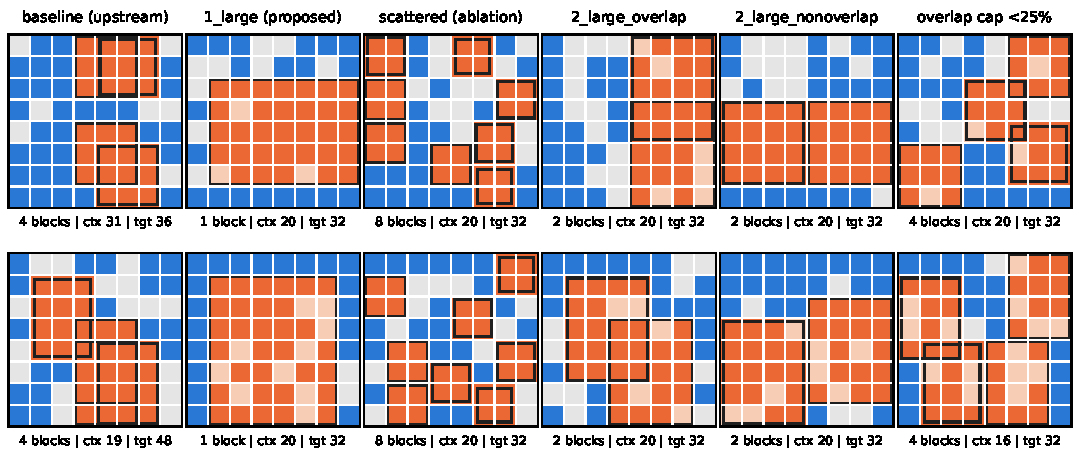
\includegraphics[width=\linewidth]{figures/fig_masks.pdf}
\caption{Two sampled masks per strategy on the $8{\times}8$ patch grid (image 0 of a batch of 64; blue: visible context,
orange: target tokens, light orange: patches of a target block not drawn as targets, grey: neither). Black boxes: the
individual target blocks; each is predicted as its own target set. Below each mask: number of target blocks, context and target tokens.}
\label{fig:masks}
\end{figure}

\begin{table*}[t]\centering\setlength{\tabcolsep}{3pt}
\caption{H1 masking strategies, 15k steps, pretraining seed 0 (validation-selected probe; test accuracy in \%). Small numbers: difference to the baseline \emph{mean over 5 seeds} (first row), coloured when it exceeds twice the baseline's seed std for that condition. Loss columns: held-out latent loss with the real context / another image's context / content-free per-position mean target. Tokens = visible context / target tokens per image; $n{\times}k$: $n$ target blocks predicted as separate sets of $k$ tokens, as upstream ($^\dagger$batch-minimum trimmed, 4--31; $^\ddagger$4 blocks, $\approx$32 distinct; $^\S$one set per 2--6-patch block). Time = training time on one L40S.}
\label{tab:h1}
\resizebox{\textwidth}{!}{\begin{tabular}{lcccccccccccc}\toprule
Strategy & Tokens & Clean & Occ 10\% & Occ 25\% & Occ 40\% & Noise .05 & Noise .15 & Loss (real/other/pos.) & Feat.\ std & Rank & Pair cos & Time (s)\\\midrule
Baseline (upstream), 5 seeds & 20$^\dagger$/45$^\ddagger$ & 48.9{\scriptsize$\pm$0.4} & 46.1{\scriptsize$\pm$0.5} & 37.3{\scriptsize$\pm$0.8} & 28.9{\scriptsize$\pm$0.4} & 45.8{\scriptsize$\pm$0.4} & 22.2{\scriptsize$\pm$1.0} & 0.150/0.402/0.278 & 0.618 & 62.9 & 0.27 & 581 \\
\textbf{1\_large}, 5 seeds & 20/32 & 49.9{\scriptsize$\pm$0.3} & 47.1{\scriptsize$\pm$0.7} & 39.6{\scriptsize$\pm$1.3} & 31.7{\scriptsize$\pm$0.5} & 46.8{\scriptsize$\pm$0.5} & 27.5{\scriptsize$\pm$2.3} & 0.132/0.399/0.269 & 0.619 & 61.2 & 0.28 & 372 \\\midrule
Baseline (upstream) & 20$^\dagger$/45$^\ddagger$ & 48.8\,{\scriptsize {\color{gray}-0.2}} & 46.4\,{\scriptsize {\color{gray}+0.3}} & 37.3\,{\scriptsize {\color{gray}+0.0}} & 28.2\,{\scriptsize {\color{gray}-0.7}} & 45.4\,{\scriptsize {\color{gray}-0.4}} & 22.0\,{\scriptsize {\color{gray}-0.2}} & 0.149/0.393/0.272 & 0.595 & 61.1 & 0.29 & 611 \\
\textbf{1\_large} (proposed) & 20/32 & 50.2\,{\scriptsize \up{+1.2}} & 46.1\,{\scriptsize {\color{gray}-0.0}} & 38.2\,{\scriptsize {\color{gray}+0.9}} & 31.4\,{\scriptsize \up{+2.5}} & 46.5\,{\scriptsize {\color{gray}+0.7}} & 31.2\,{\scriptsize \up{+9.0}} & 0.128/0.357/0.244 & 0.550 & 60.6 & 0.34 & 549 \\
\textbf{scattered} (ablation) & 20/32--36$^\S$ & 50.1\,{\scriptsize \up{+1.1}} & 46.3\,{\scriptsize {\color{gray}+0.3}} & 38.2\,{\scriptsize {\color{gray}+0.9}} & 30.3\,{\scriptsize \up{+1.5}} & 41.7\,{\scriptsize \dn{-4.1}} & 17.0\,{\scriptsize \dn{-5.2}} & 0.113/0.265/0.180 & 0.290 & 62.6 & 0.58 & 852 \\
\midrule
2\_large\_overlap & 20/2$\times$16 & 51.8\,{\scriptsize \up{+2.9}} & 48.9\,{\scriptsize \up{+2.8}} & 37.7\,{\scriptsize {\color{gray}+0.5}} & 27.7\,{\scriptsize \dn{-1.2}} & 47.0\,{\scriptsize \up{+1.2}} & 22.0\,{\scriptsize {\color{gray}-0.2}} & 0.142/0.381/0.265 & 0.588 & 60.4 & 0.31 & 541 \\
2\_large\_nonoverlap & 20/2$\times$16 & 49.8\,{\scriptsize \up{+0.9}} & 47.2\,{\scriptsize \up{+1.1}} & 34.1\,{\scriptsize \dn{-3.2}} & 25.2\,{\scriptsize \dn{-3.7}} & 45.4\,{\scriptsize {\color{gray}-0.3}} & 22.8\,{\scriptsize {\color{gray}+0.6}} & 0.150/0.379/0.264 & 0.621 & 58.7 & 0.31 & 566 \\
overlap cap $<$25\% & 16.8/4$\times$8 & 50.3\,{\scriptsize \up{+1.4}} & 46.1\,{\scriptsize {\color{gray}+0.0}} & 37.1\,{\scriptsize {\color{gray}-0.1}} & 27.4\,{\scriptsize \dn{-1.5}} & 47.4\,{\scriptsize \up{+1.6}} & 21.5\,{\scriptsize {\color{gray}-0.7}} & 0.146/0.380/0.265 & 0.582 & 60.2 & 0.30 & 516 \\
\bottomrule\end{tabular}}\end{table*}


%=====================================================================================================
\section{Controlled comparison (Part C) and why each geometry did (not) help}
\label{sec:partc}
All runs share the splits, corruption tensors, probe protocol, evaluation seeds, 15k steps, data order and parameter count
(1{,}412{,}864); only the mask sampler differs (Tab.~\ref{tab:h1}). The baseline was trained with 5 pretraining seeds, so
its seed standard deviation is known: 0.4 (clean), 0.8 (occ 25\%), 0.4 (occ 40\%), 1.0 ($\sigma{=}0.15$) points.

\begin{figure*}[t]
\centering
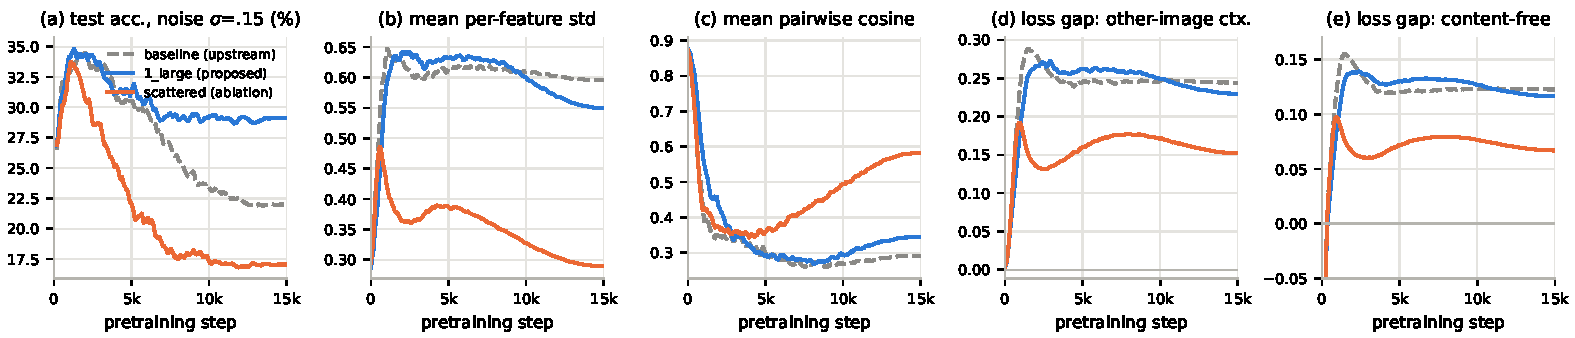
\includegraphics[width=\linewidth]{figures/fig_h1_mech.pdf}
\caption{Why one large target block is the most noise-robust geometry and scattered small blocks the least (seed 0, fixed
probe, 250-step moving average of the evaluations every 50 steps). (a) Test accuracy at noise $\sigma{=}0.15$. (b--c) Collapse
diagnostics of the pooled clean test features. (d) Held-out latent loss with another image's context minus the loss with the
image's own context: how much the prediction depends on the image's own content. (e) Loss of the content-free per-position
mean target minus the real-context loss: how much better than a position-only guess the predictor is.}
\label{fig:h1mech}
\end{figure*}

\textbf{Proposed: one large block (\texttt{1\_large}) -- the most noise-robust geometry.}
\obs Over 5 pretraining seeds 1\_large reaches \textbf{27.5$\pm$2.3} at $\sigma{=}0.15$, against 22.2$\pm$1.0 for the baseline
(+5.3 points, the largest gain of any masking geometry). 
% It keeps 55\% of its clean accuracy under $\sigma{=}0.15$
% (baseline 45\%, the other fixed-count samplers 42--46\%, scattered 34\%), and 
Its noise accuracy stops falling after
$\approx$6k steps while the baseline's keeps falling to the end (Fig.~\ref{fig:h1mech}a). Clean and occlusion accuracy
improve as well: 49.9$\pm$0.3 clean, 39.6$\pm$1.3 at 25\% and 31.7$\pm$0.5 at 40\% occlusion, i.e.\ +0.9, +2.3 and +2.8 points
over the baseline's 5-seed mean, each larger than both seed standard deviations. Its features keep the baseline's spread
(per-feature std 0.619 vs 0.618, pairwise cosine 0.29 vs 0.27, 5 seeds), and its prediction depends at least as much on
the image's own content: the loss rises by 0.267 when the context is taken from another image (baseline 0.252) and the
content-free target is 0.138 above the real-context loss (baseline 0.127; Fig.~\ref{fig:h1mech}b--e).
\interp With one contiguous hole of 35--42 patches the visible context is a ring around it, and most target tokens are
several patches away from any visible patch. The predictor can neither copy neighbouring texture nor fall back on the
target positions; it has to infer the hidden region from what the image shows as a whole (object, layout, colour). This
pushes the context encoder towards image-level, more semantic features, which i.i.d.\ pixel noise disturbs less than the
local detail it destroys. The same structure (``infer a large missing region from distant, peripheral context'') is what
the occlusion test asks. 
% The paper's principle that targets must be large enough to be semantic~\cite[Tab.~8]{assran2023ijepa}
% is about \emph{relative} scale: a CIFAR object fills most of a $32{\times}32$ frame, so the default $3{\times}3$-patch blocks
% ($12{\times}12$ px) are closer to object parts or texture, and a block covering half the image is closer to the object scale
% (\spec this would explain why larger-than-default targets help here but hurt on ImageNet, Tab.~8 of~\cite{assran2023ijepa}).
Two limits remain. Noise still moves the features as much as for the baseline (clean--noisy cosine 0.71 vs 0.71); what
improves is how much class information survives the shift. And 27.5\% is only at the level of a frozen random encoder
(26.6$\pm$1.3): the geometry slows the decline but does not make the encoder noise-invariant (that needs
Sec.~\ref{sec:noise}). On occlusion the contrast with the ablation is weaker than on noise: scattered (one seed) reaches
38.2/30.3 at 25/40\%, against 38.2/31.4 for 1\_large with the same seed, so H1's occlusion gain is only partly due to
contiguity. This is because in the ablation, we maintain that we should atleast get 20 context patches and 32 target patches 
after masking. So downstream occlusion performance does not vary much.

\textbf{Ablation: scattered small blocks -- local features, a position shortcut and the worst noise robustness.}
\obs Clean accuracy (50.1) and occlusion are unaffected, but $\sigma{=}0.05$ falls to 41.7 ($-$4.1) and $\sigma{=}0.15$ to
\textbf{17.0} ($-$5.2), the lowest of all runs (34\% of clean). The collapse diagnostics show why
(Fig.~\ref{fig:h1mech}b--c): from $\approx$1k steps on, the mean per-feature std stays at about half the baseline's
(0.290 vs 0.618 at 15k) and the mean pairwise cosine doubles (0.58 vs 0.29), while the effective rank stays high (62.6),
so this is not dimensional collapse. The content-ablated held-out losses (Fig.~\ref{fig:h1mech}d--e) are much closer to
the real-context loss: taking the context from another image raises the loss by only 0.152 (baseline 0.252, 1\_large 0.267),
and the content-free per-position mean target is only 0.067 above it (baseline 0.127, 1\_large 0.138).
\interp Every 2--6-patch target has visible context one patch away, so the predictor can solve the task from the target
\emph{positions} plus interpolation of neighbouring patches: the image's own content matters less (small other-image gap)
and a position-only guess is already close (small content-free gap). The context encoder is pushed towards local,
high-frequency patch detail with little image-level variation. Writing each pooled feature as a shared offset $m$ (the
mean over images) plus an image-specific deviation $v_i$, we measured $\lVert m\rVert{=}4.35$ (baseline) vs 3.91
(scattered) but an RMS deviation of 6.82 vs 3.33: the offset changes little and the image-specific part halves.
Per-feature std ignores $m$ and halves with $v$; the mean pairwise cosine is $\approx\lVert m\rVert^2/\mathbb E\lVert f\rVert^2$
(0.29 vs 0.58 measured), so it doubles. Because the probe standardises features, clean accuracy is unaffected, but pixel noise
destroys exactly the local detail these features encode and moves them far relative to the small differences between
images. 
% This matches the paper's finding that \texttt{random} patch targets give much less semantic features (17.6 vs
% 54.2,~\cite[Tab.~6]{assran2023ijepa}).

\textbf{Two large blocks.} Predicted as two separate sets of 16, \texttt{2\_large\_overlap} (two 16--30-patch blocks) is the
best single-seed run on clean (51.8, +2.9) and 10\% occlusion (48.9, +2.8) but not at 25/40\% occlusion (+0.5/$-$1.2) or
$\sigma{=}0.15$ (22.0). 
% (When both blocks were predicted as one 32-token set, i.e.\ as one large region, it had reached
% 40.0/30.9 at 25/40\% occlusion; \texttt{results/h1\_perblock}.) 
\texttt{2\_large\_nonoverlap} loses $-$3.2/$-$3.7 at 25/40\%
occlusion. 
% Two disjoint blocks of 16--20 patches that still leave 20 context patches fit on the $8{\times}8$ grid almost only as
% full-width or full-height bands (6.6 position draws per image and 0.13 block-size redraws per batch; Fig.~\ref{fig:masks}),
% so every target row or column borders a context band. \spec The task again becomes one-dimensional interpolation between
% neighbouring bands, and the model never has to infer a compact central region, which is what the occlusion test removes.

\textbf{Capped overlap between the 4 small blocks.} The overlap cap ($|A\cap B|/|A|<0.25$ for every pair) gains slightly
on clean (+1.4) but loses at 40\% occlusion ($-$1.5) and reaches only 21.5 at $\sigma{=}0.15$. 

\spec In the two large block experiments and the capped overlap experiment, although the experiments were run with only one 
seed, the downstream results do not differ much from the baseline results, since we maintain the context and token patch budgets
in all the experiments. These masking strategies still allow for context patches from the central region (the object region)
to be sampled during training, similar to the baseline masking strategy. Due to this we do not observe much differences in the 
results.

% Spreading the four small
% blocks apart does not change \emph{what} is predicted \emph{from what}: each block still has context next to it. The cap
% also lowers the context to 16.8 tokens (a 3$\times$4 batch almost always contains an image with only 16 available), with no
% measurable effect, so the context size in the 16--20 range is not limiting.

\textbf{Cost.} No sampler changes the parameter count (1{,}412{,}864). Training takes 516--566\,s per 15k steps on one L40S for the fixed-count samplers (baseline 581\,s)
and peak GPU memory is 0.26\,GB for them vs 0.33\,GB for the baseline, except for scattered, which makes
one predictor call per small block (6--16 per step): 852\,s and 0.51\,GB. Sampling costs 2--5\,ms per batch on the CPU.


%=====================================================================================================
\section{Targeted fix for the failure mode: noise on the context input}
\label{sec:noise}
\textbf{Hypothesis (H3).} If the noise failure is a missing invariance rather than missing information
(Sec.~\ref{sec:failure}), then feeding the \emph{context} encoder noisy images while the EMA target encoder keeps the clean
image should make the evaluated encoder noise-invariant. \emph{Prediction:} with the standard clean-trained probe, accuracy
at $\sigma{=}0.15$ exceeds both the baseline and the random encoder by more than the seed std, and clean accuracy drops by
less than 1.4 points. \emph{Falsified} otherwise. \emph{Ablation:} $p{=}0$, which is bit-identical to the baseline (tested).

\textbf{Change.} After the upstream augmentation, each pretraining image is noised with probability $p{=}0.5$ with its own
$\sigma\sim U(0,0.2)$, in $[0,1]$ space, clipped and re-normalised exactly like the test noise (App.~\ref{app:diff}); the noise
uses its own seeded generator, disjoint from the test-corruption seeds. Only the context encoder sees the noisy copy; masks,
loss, targets and data order are unchanged. Parameters, step time (587\,s per 15k steps vs 556--611\,s for the baseline seeds)
and peak memory (0.33\,GB) are unchanged.

\begin{figure}[t]
\centering
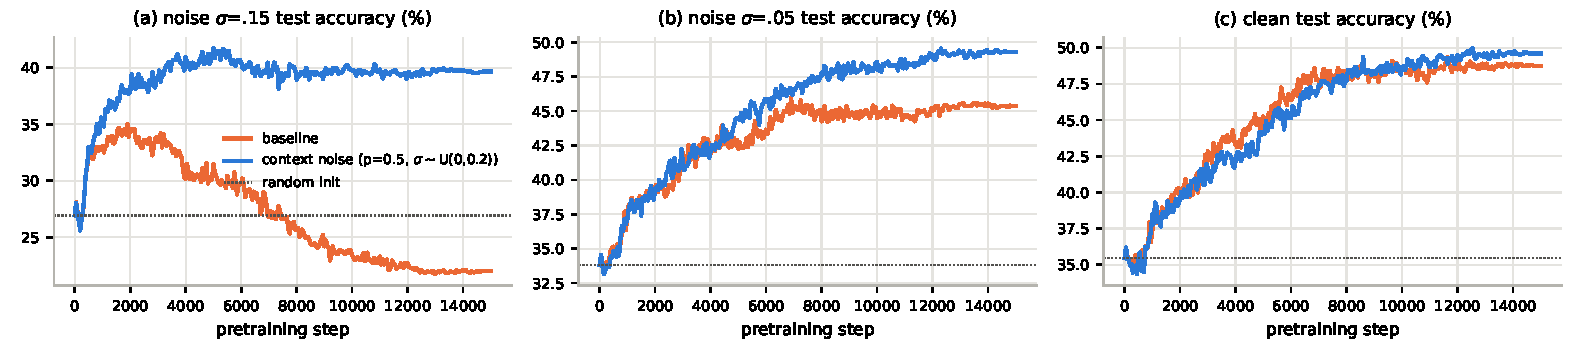
\includegraphics[width=\linewidth]{figures/fig_noise.pdf}
\caption{Test accuracy during pretraining (fixed clean-trained probe, seed 0) for the baseline and for pretraining with
noise on the context-encoder input. Dotted: the step-0 (random) encoder.}
\label{fig:noise}
\end{figure}

\begin{table}[t]\centering\small\setlength{\tabcolsep}{3.2pt}
\caption{The noise failure and two remedies (test accuracy, \%, 15k steps). Rows 3--4: the \emph{frozen} encoder (seed 0) with a \emph{mixed-trained} probe: every epoch each probe-train image is clean or, with probability $\tfrac12$, a fresh $\sigma{=}0.15$ noisy copy; $(\mathrm{lr},\mathrm{wd})$ chosen on the mean of clean and noisy validation accuracy. Row 5: pretraining with noise on the context-encoder input only ($p{=}0.5$, $\sigma\sim U(0,0.2)$), evaluated with the standard clean-trained probe; its ablation ($p{=}0$) is row 1. cos$_{.15}$: mean cosine between the clean and $\sigma{=}0.15$ features of the same test image.}
\label{tab:noise}
\begin{tabular}{lccccccc}\toprule
Encoder / probe & Clean & Occ 10\% & Occ 25\% & Occ 40\% & Noise .05 & Noise .15 & cos$_{.15}$ \\\midrule
Baseline, clean probe (5 seeds) & 48.9{\scriptsize$\pm$0.4} & 46.1{\scriptsize$\pm$0.5} & 37.3{\scriptsize$\pm$0.8} & 28.9{\scriptsize$\pm$0.4} & 45.8{\scriptsize$\pm$0.4} & 22.2{\scriptsize$\pm$1.0} & 0.71 \\
Random init, clean probe (5 seeds) & 35.1{\scriptsize$\pm$0.3} & 34.1{\scriptsize$\pm$0.9} & 29.6{\scriptsize$\pm$0.6} & 23.9{\scriptsize$\pm$0.7} & 34.2{\scriptsize$\pm$0.8} & 26.6{\scriptsize$\pm$1.3} & 1.00 \\\midrule
Baseline (s0), \emph{mixed-trained probe} & 48.8 & 46.3 & 35.8 & 27.7 & 48.1 & 39.6 & -- \\
Random init (s0), \emph{mixed-trained probe} & 34.5 & 33.3 & 28.2 & 24.1 & 34.3 & 31.3 & -- \\
\midrule
\textbf{Context-noise pretraining} (s0), clean probe & 47.5 & 46.0 & 38.4 & 29.9 & 47.6 & 41.9 & 0.95 \\
\bottomrule\end{tabular}\end{table}


\obs (Tab.~\ref{tab:noise}, Fig.~\ref{fig:noise}.) Accuracy at $\sigma{=}0.15$ rises to $\approx$41\% by step 5k and stays there
(41.9\% at 15k, +19.7 over the baseline's 5-seed mean and +15.3 over the random encoder); $\sigma{=}0.05$ improves by +1.8 and
the occlusion levels change by $-$0.1 to +1.2 (within or near seed noise). Clean accuracy is 47.5\% with the validation-selected probe ($-$1.4) and 49.6\% with
the fixed probe used for the curves (baseline seed 0: 48.8). The clean cost is therefore 1.4 points under the selected probe 
% (about 3 baseline seed standard deviations, at the edge of H3's 1.4-point tolerance) 
and none under the fixed probe: a small but probably real cost. The clean--noisy feature cosine rises from 0.71 to 0.95 while the effective rank stays high (57.7): the features are
stable \emph{and} informative. Single seed; the $\sigma{=}0.15$ gain is $\approx$20 baseline standard deviations.

\interp This is denoising~\cite{vincent2008denoising} carried out in latent space: to predict the clean target features from
a noisy context, the context encoder must map a noisy patch to (nearly) the features of its clean version, so the
noise-sensitive directions that grow during baseline training are suppressed in the evaluated encoder. Keeping the target
clean matters by design: a noisy target would ask the predictor to reproduce the noise. The I-JEPA paper deliberately avoids
hand-crafted augmentations because they bake in invariances that may not suit every task~\cite[Sec.~1]{assran2023ijepa}; our
result is the other side of that choice: without some invariance pressure, a robustness that the probe needs does not appear
by itself. \textbf{H3 is supported} on this condition. Whether the invariance generalises to corruptions not seen in
pretraining is untested (Sec.~\ref{sec:answers}).

% \textbf{Mixed probe on the noise-pretrained encoder.} The diagnostic of Sec.~\ref{sec:failure} on this encoder: the mixed-trained probe
% reaches 45.5\% at $\sigma{=}0.15$ (baseline encoder: 39.6\%) and 49.2\% clean, so only a small shift remains.


%=====================================================================================================
\section{Answers to the assignment questions}
\label{sec:answers}
\begin{description}[leftmargin=0pt,itemsep=2pt]
\item[Does lower prediction loss correspond to better features?] No. Within a run the held-out loss is minimal at step 700,
when accuracy and rank are still at random-encoder level, and then \emph{rises} while accuracy improves by 13 points.
% ($\rho{=}{+}0.65$ between loss and validation accuracy after step 500). 
The 500-step model has the lowest loss of the Part~A
checkpoints (0.078) and random-level features. 
After the initial drop in the training loss, the loss starts increasing due to the target encoder shifting away from 
position-dependent features towards semnatic concepts making it harder for the context encoder and the predictor to learn.
This forces the context encoder to learn useful contextual and semantic features from the availabel context features, 
for the predictor to predict the hidden target features. This is supported by the increasing gaps between the validation 
heldout latent loss, context-free loss and other-image context loss.
% Across variants the lowest loss belongs to
% scattered (0.113), the least noise-robust run (17.0 at $\sigma{=}0.15$). The early drop is learnt from positions: the loss with another image's
% context falls exactly like the real-context loss, and a content-free per-position predictor beats both until step 250
% (Sec.~\ref{sec:h2}). The effective rank, by contrast, tracks clean accuracy.
%  ($\rho{=}{+}0.92$).

\item[Does the change improve clean classification, occlusion robustness, or both?] The geometry change 
(1\_large) is the most
noise-robust geometry ($27.5{\pm}2.3$ vs $22.2{\pm}1.0$ at $\sigma{=}0.15$, 5 seeds each) and improves occlusion robustness
(+2.3 / +2.8 points at 25 / 40\%) with a small clean gain (+0.9); it slows the noise failure but does not repair it (it stays
at random-encoder level). Pretraining with context noise repairs the noise failure (+19.7 at $\sigma{=}0.15$) at a small clean cost ($-$1.4 with the
selected probe) and leaves occlusion unchanged. 
% Neither closes the gap to the oracle probe at 40\% occlusion (38.4\%), which
% is the part of the drop due to a feature shift rather than to missing evidence.

\item[Are gains caused by mask geometry, or by a change in visible/target counts?] By geometry. All H1 candidates use exactly
20 context and 32 target tokens per image (scattered: 32--36), and the scattered
ablation with the same counts is the least noise-robust run (17.0 vs $27.5{\pm}2.3$ for 1\_large at $\sigma{=}0.15$), with
halved image-specific feature variance and a held-out loss close to a position-only prediction. On occlusion the separation
is weaker (scattered, one seed, matches 1\_large at 25\% and is 1.1 points lower at 40\%), so the occlusion gain is only
partly due to contiguity. Within ``geometry'',
contiguity and block scale are confounded (1\_large has one large contiguous block, scattered many small ones).

\item[Could extra parameters, different training exposure, or a probe change explain the result?] No for parameters: every
run has 1{,}412{,}864 trainable parameters. No for exposure: same 15k steps, same seeded data order and images, and the
predictor sees fewer target tokens than the baseline (32 vs 45). No for the probe: identical protocol, $(\mathrm{lr},\mathrm{wd})$
selected on validation; the same ranking holds under the fixed probe setting (e.g.\ 1\_large 51.0 clean / 31.5 at 40\%
occlusion, baseline 48.8 / 28.2). According to the paper, increasing the depth of the predictor can help with improved 
downstream performance, but significant changes can only be seen when training on larger image sizes and larger dataset size.
% For context noise the extra exposure \emph{is} the mechanism; its noise is drawn from a
% range chosen knowing the strongest test level ($\sigma_{\max}{=}0.2>0.15$), with seeds disjoint from the test noise.

\item[Could apparent feature stability come from collapsed or uninformative representations?] Yes, and this is observed in 
the training loss graph where the loss initially drops and the heldout losses (context free, and other image's context) drop
converge. At this point, the features are collapsed since they context encoder and predictor depend on the target positions
to predict the target features and the target encoder's weights are still not fully changed from its random weights. But as
the training proceeds, the target encoder shifts away and produces high image and patch variant target features, forcing the 
context encoder and predictor to move beyond just depending on the target position embeddings and focus on contextual and 
semantic concepts in the image. 

% Yes, and the random encoder is
% the clearest case: its features are the most stable under noise (clean--noisy cosine 0.997) and the least informative
% (35\% clean). The baseline's stability falls as its rank grows (cosine 0.71 at 15k). Stability is only meaningful together
% with rank and accuracy: context-noise pretraining is stable (0.95) \emph{and} informative (rank 57.7, 47.5\% clean). Scattered
% masking shows the opposite pitfall: high pairwise cosine (0.60) from a halved image-specific variance without loss of rank.

\item[Which single follow-up experiment would you prioritise with one more week?] To evaluate the pretrained encoders on low-level
vision tasks like counting and segmentation and study the performance. To also scale the image size and dataset size to large datasets,
and scale the encoder and predictor sizes, to study how it improves downstream performance and in which scenarios its features can collapse.
% Evaluate context-noise pretraining (3 seeds,
% combined with and without 1\_large) on corruptions it never saw, at a maximum training noise \emph{below} the test level
% ($\sigma_{\max}{=}0.1$) and on other families (blur, JPEG, impulse noise, contrast; the standard CIFAR-10-C set). If robustness
% transfers, the diagnosis ``missing invariance pressure'' is confirmed and the fix is a method; if it only helps at the trained
% $\sigma$, it is test-condition matching. This single experiment decides which of the two the noise result is.
\end{description}

\subsection*{Final research question: what limits robust representation learning here?}
% Pretraining with only the initial training budget of 500 steps limits the encoder from learning any useful features and results in 
% poor downstream performance. 
\begin{itemize}
\item \textbf{Image size} The small image size $32\times32$ limits different masking patterns and strategies when experimenting with larger target blocks.
\item \textbf{Not feature collapse.} Every run ends with effective rank 57--66, top-1 singular-value share $\le$0.16 and growing
feature spread; the one contraction we found (scattered) leaves the rank intact.
\item \textbf{Not context size or target overlap.} Lowering the context to 16.8 tokens and capping the overlap between the
4 small blocks change accuracy by at most 1.5 points.
\item \textbf{Mask geometry decides what the encoder relies on.} Large targets far from the context keep image-level
features and the best noise robustness of any geometry (1\_large, +5.3 points at $\sigma{=}0.15$); small targets next to the
context produce local, position-driven features and the worst (scattered, $-$5.2). Geometry alone does not make the encoder
noise-invariant, and adds $\approx$3 points under 40\% occlusion.
\item \textbf{Limited training is the bottleneck only at the assignment budget.} At 500 steps the encoder equals a random encoder;
longer training improves clean accuracy but \emph{worsens} noise robustness.
\item \textbf{Best-supported explanation: the objective has no invariance pressure, and a clean-only probe protocol exposes it.}
I-JEPA's target is the clean image's own features, so the encoder grows features for fine local structure that noise
perturbs; the class information survives (39.6\% with a probe trained on mixed clean and noisy images) but moves in feature space. Putting the
perturbation on the context side alone recovers it (41.9\% with the clean probe). For occlusion the largest part of the drop
is missing evidence (the supervised reference loses the same fraction).
\item \textbf{Next experiment:} Scaling the image and dataset sizes, scaling the encoder and predictor networks, 
and measure the feature robustness against noise, occusion. To also evaluate the features on low-level vision tasks.
\end{itemize}


\section{Limitations}
\begin{itemize}
\item Most Part B/C variants have one pretraining seed; the 1\_large and baseline estimates use 5 seeds. In particular the
1\_large vs scattered noise contrast compares 5 seeds (25.0--31.2\% at $\sigma{=}0.15$) with one scattered seed (17.0\%).
\item The mechanism (image-level vs local and positional prediction) is inferred from the collapse and held-out-loss
diagnostics (Fig.~\ref{fig:h1mech}); no run intervenes on it directly. Effects below
$\approx$1.5 points (clean, occlusion) or $\approx$3 points ($\sigma{=}0.15$, seed std 1.0 for the baseline and 2.3 for 1\_large) are not resolved.
\item Every comparison uses 15k steps, 30$\times$ the assignment's 500; at 500 steps no variant learns useful features.
Hyper-parameters were not re-tuned for any variant.
\item \texttt{ctx\_noise} uses $\sigma_{\max}{=}0.2$, chosen knowing the strongest test noise is 0.15; it was not tuned on
test accuracy, but its robustness to \emph{other} corruptions is untested.
\item The linear probe is fit on only 2{,}000 images; CIFAR-10 at $32{\times}32$ with 64 tokens is far from the paper's setting.
\end{itemize}

\section*{Reproducibility, attribution and AI disclosure}
Upstream: \texttt{keon/jepa} @ \texttt{d55bab7b} (MIT), model code copied verbatim into \texttt{models/modified\_ijepa.py}.
Every run: \texttt{bash scripts/train.sh configs/<experiment>.yaml [k]} then \texttt{bash scripts/evaluate.sh runs/<name>\_s<k>}
(mask samplers bit-identical to the notebooks in which the experiments were developed; the evaluation reproduces the
stored results exactly). Seeds: splits 0/1,
corruptions 1000--1011, probe 0, held-out masks 12345, pretraining 0 (and 1--4 where stated), context noise 50000+seed.
Hardware: NVIDIA L40S (runs) and RTX 2080 Ti (interactive). An AI assistant (Claude, Anthropic) was used to build the
mask strategies, the helper functions and the downstream evaluation; every result was produced by the code in the
repository and checked against the notebooks.

{\small
\bibliographystyle{unsrtnat}
\bibliography{refs}
}

\appendix
\section{Code changes}
\label{app:diff}
\textbf{Code diff.} \texttt{models/modified\_ijepa.py} is upstream \texttt{ijepa.py} with only \texttt{train()} changed
(\texttt{diff ../jepa/ijepa.py models/modified\_ijepa.py}); \texttt{Encoder}, \texttt{Predictor},
\texttt{sample\_ijepa\_masks}, \texttt{ema\_update} and the loss formula are unchanged. The training step:
\begin{lstlisting}
for step in range(steps):                                            # was: for epoch ... for imgs, _ in loader
    imgs = next(it)                                                  # seeded reshuffle of the 10k split per epoch
    cl, tls, cols = mask_fn(imgs.size(0), ctx_enc.grid, rng)         # was: sample_ijepa_masks(...)  (models/masks.py)
    ci = torch.tensor(cl, device=device); tis = [torch.tensor(t, device=device) for t in tls]
    cols = cols or [slice(None)] * len(tis)                          # per-target context subset (all for the reported samplers)
    ctx_imgs = add_context_noise(imgs, noise_gen, p, sigma_max) if ctx_noise else imgs  # H3: targets clean
    with torch.no_grad(): full = F.layer_norm(tgt_enc(imgs), (D,))  # unchanged: stop-gradient target
    ce = ctx_enc(ctx_imgs, ci)
    loss = sum(F.smooth_l1_loss(pred(ce[:, c], ci[:, c], ti), full.gather(1, ti.unsqueeze(-1).expand(-1, -1, D)))
               for c, ti in zip(cols, tis)) / len(tis)
    opt.zero_grad(); loss.backward(); opt.step(); ema_update(tgt_enc, ctx_enc, m)   # unchanged
\end{lstlisting}
\textbf{Fixed-count rule} (\texttt{models/masks.py}, \texttt{blocks}; condensed). The upstream strategy is still the
default and is tested to reproduce \texttt{sample\_ijepa\_masks} exactly.
\begin{lstlisting}
def blocks(B, grid, rng, ctx_size=20, tgt_size=32, n_targets=4, tgt_scale=(0.15, 0.20), ..., overlap=True):
    for _ in range(max_geom_tries):
        th, tw = _bsize(grid, rng.uniform(*tgt_scale), rng.uniform(*tgt_aspect))   # one shape per batch (as upstream)
        ch, cw = _bsize(grid, rng.uniform(*ctx_scale), 1.0)
        for b in range(B):
            for _ in range(max_draw_tries):                           # redraw POSITIONS until the counts fit
                union, blks = _place_blocks(grid, rng, th, tw, n_targets, overlap, tgt_size)  # n = 0: until >= tgt_size
                if union.bit_count() < tgt_size: continue
                c = rng.choice(_block_bits(grid, ch, cw)) & ~union     # context block minus ALL target patches
                if c.bit_count() < ctx_size: continue
                ctx_list.append(_take(rng, _bits_to_idx(c), ctx_size))          # uniform subset, exact count
                tgt_sets.append([_take(rng, _bits_to_idx(t), tgt_size // len(blks)) for t in blks])  # one set per block
                break
            else: break                                               # redraw the batch's block sizes
        if len(ctx_list) == B: return ctx_list, list(zip(*tgt_sets))   # n target sets of 32/n tokens (as upstream)
\end{lstlisting}
\textbf{Configs.} An experiment names a mask-strategy file whose arguments are the strategy's defaults:
\begin{lstlisting}
# configs/proposed.yaml           # configs/masks/1_large.yaml        # configs/masks/scattered.yaml (ablation)
base: baseline.yaml               strategy: blocks                    strategy: scattered
name: proposed                    ctx_size: 20                        ctx_size: 20
mask: masks/1_large.yaml          tgt_size: 32                        tgt_size: 32
                                  n_targets: 1                        tgt_scale: [0.04, 0.07]
# configs/ctx_noise.yaml          tgt_scale: [0.52, 0.62]
base: baseline.yaml               # other files: 2_large_overlap, 2_large_nonoverlap,
ctx_noise: {p: 0.5, sigma_max: 0.2, seed: 50000}   # overlap_frac
\end{lstlisting}
\textbf{Context noise} (\texttt{add\_context\_noise}): with probability $p{=}0.5$ an image gets $\sigma\sim U(0,0.2)$ Gaussian noise in $[0,1]$
space, clipped and re-normalised exactly like the test noise, from its own seeded generator.


\section{Automated checks}
\label{app:tests}
\textbf{pytest} (\texttt{tests/}, 49 tests, all passing on CPU in $\approx$12\,s): for every mask-strategy file, valid and
disjoint context/target indices, the declared token counts at batch sizes 1/16/64 and determinism given a seed; the
\texttt{upstream} strategy equals \texttt{sample\_ijepa\_masks} exactly; with \texttt{per\_block} every target set lies inside one block, and \texttt{per\_block: false}
gives one set drawn from the union; the overlap cap holds;
the leak guard detects an injected overlap; after one training step the target encoder equals
$m\,\bar\theta_0+(1-m)\,\theta_1$ exactly, receives no gradient, and $m{=}1$ freezes it; shapes and finite outputs; the
context encoding does not depend on target pixels; context noise is seeded and leaves non-noised images unchanged;
a 2-step CPU smoke run of every experiment config; splits disjoint, sized and deterministic; corruptions paired and in
range; probe selection leaves the encoder's parameter hash unchanged. Equivalence with the notebooks: with \texttt{per\_block: false} all mask
configs give bit-identical masks to the notebook samplers (300 batches each), and \texttt{evaluate.py} on the
notebook checkpoints reproduces every stored metric to $10^{-6}$.

\textbf{Notebook assertions} (run on every execution): section-10 sanity checks (sampler $=$ upstream, shapes, stop-gradient,
EMA, frozen probe, identical splits/corruption seeds); for each new sampler: exact token counts at batch sizes 1/7/64, no
context/target overlap, rectangles of the intended size inside the intended region, overlap rules checked by brute force,
sampled layout distribution equal to an independent rejection sampler (total-variation distance at the sampling-noise
level); context noise: $p{=}0$ is bit-identical to the baseline, noised fraction 0.496, mean $\sigma$ 0.099, measured
pixel noise / $\sigma$ = 0.996, target encoder input equals the clean batch, and the step-by-step loop equals
\texttt{pretrain()} to $3{\cdot}10^{-8}$ including after a stop/resume.


\clearpage
\makeatletter\setlength{\@fptop}{0pt}\makeatother   % float pages: figures at the top
\section{Training curves of all runs}
\label{app:curves}
The graphs printed during training (the notebooks' \texttt{plot\_training}, \texttt{plot\_metrics} and
\texttt{plot\_robustness\_curves}) for every 15k-step, seed-0 run of Table~\ref{tab:h1} and the context-noise run of
Sec.~\ref{sec:noise}, one curve per run in every panel. The evaluation curves use the fixed probe setting
(lr $3{\cdot}10^{-3}$, wd $10^{-4}$) every 50 steps, so they are descriptive only; the reported numbers use the
validation-selected probe. Step 0 is the random initialisation.

\begin{figure}[!ht]
\centering
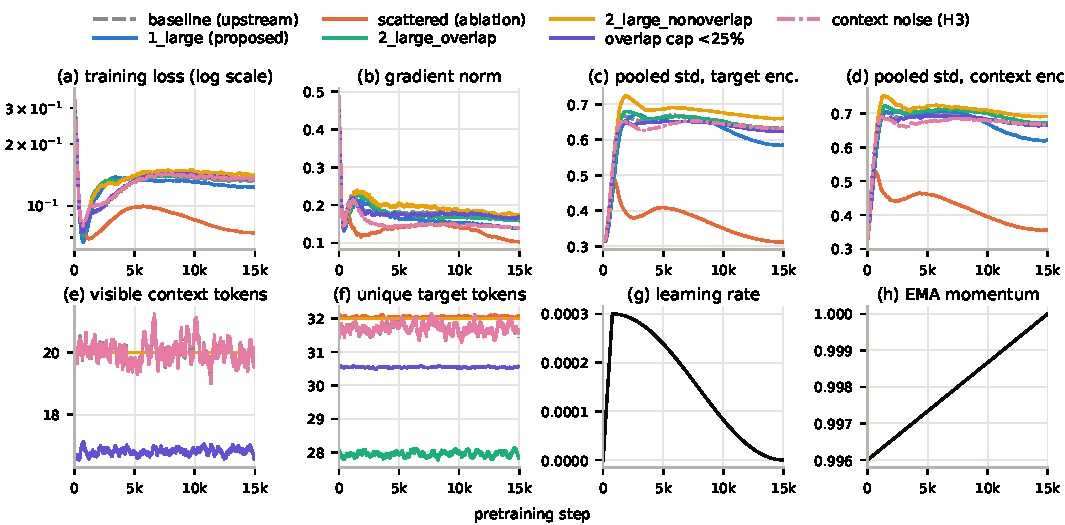
\includegraphics[width=\linewidth]{figures/fig_app_training.pdf}
\caption{Training signals, logged every step (moving average over 300 steps). (c)--(d) std over the batch of the
mean-pooled tokens, averaged over the 128 dimensions; (d) for context noise is measured on the noised context input.
(e) context tokens after the batch-minimum trim; (f) distinct target patches per image (a patch covered by two blocks
counts once). Baseline and context noise use identical masks, so their curves coincide in (e)--(f).
(g)--(h) the same schedule for every run. The per-block runs (scattered, 2\_large, overlap cap)
were trained before (b)--(d) and (f) were logged; their curves come from a retraining with the same seed and config.}
\label{fig:app_training}
\end{figure}

\begin{figure}[!ht]
\centering
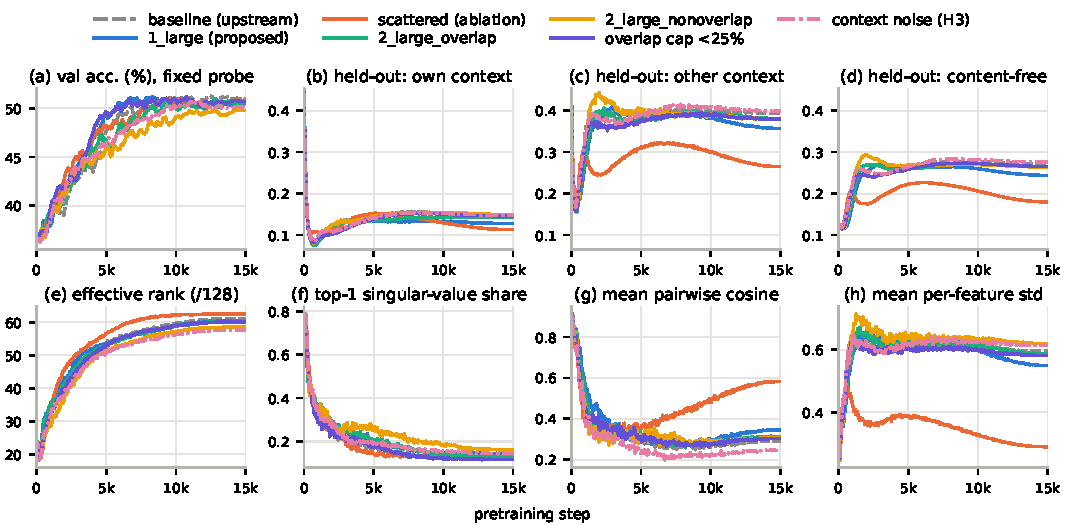
\includegraphics[width=\linewidth]{figures/fig_app_metrics.pdf}
\caption{Periodic evaluation (every 50 steps). (a) validation accuracy of the fixed probe (moving average over 5
evaluations). (b)--(d) held-out latent loss (``held-out'') on the validation images with fixed upstream masks (seed 12345): with the
image's own context, with another image's context, and for the content-free per-position mean target; the three
panels share one y-range. (e)--(h) collapse statistics of the pooled clean test features.}
\label{fig:app_metrics}
\end{figure}

\begin{figure}[!ht]
\centering
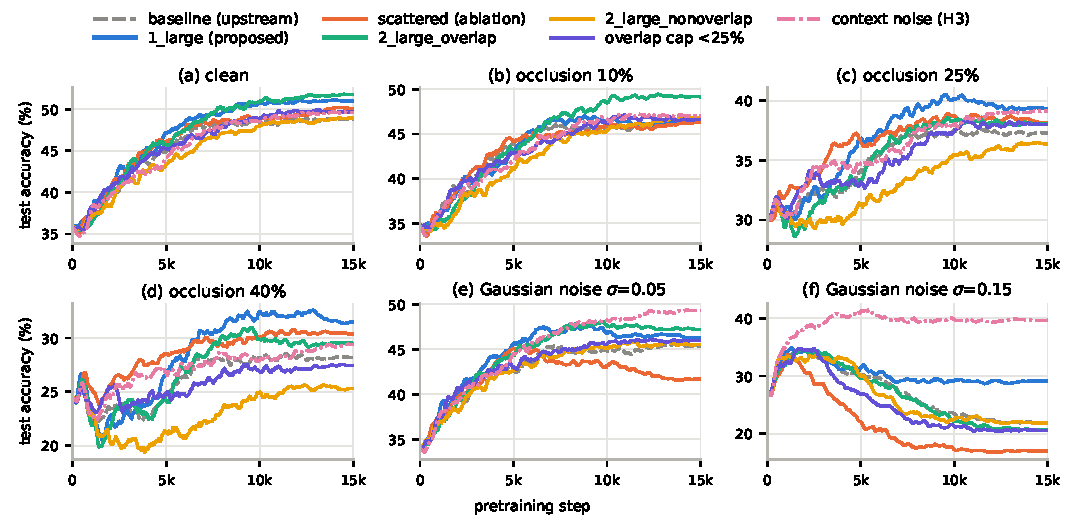
\includegraphics[width=\linewidth]{figures/fig_app_robustness.pdf}
\caption{Test accuracy per condition with the fixed clean-trained probe (moving average over 5 evaluations; chance is 10\%). Descriptive only, never used for selection.}
\label{fig:app_robustness}
\end{figure}


\end{document}
